\section{Use Case Diagram}

\begin{figure}[H]
    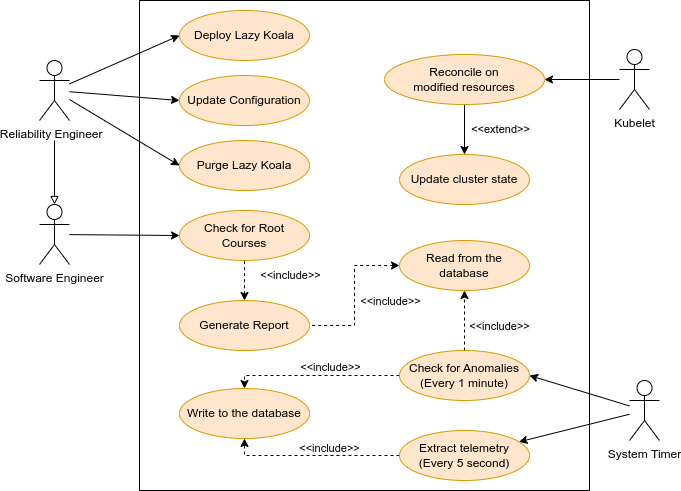
\includegraphics[width=15cm]{assets/requirement-specification/use-case.png}
    \caption{Use case diagram (self-composed)}
    % \label{fig:poc-autoencoder}
\end{figure}


\newcommand{\UseCaseDescription}[9]{
    \textbf{}
    \begin{longtable}{|p{40mm}|p{113mm}|}
    \hline
        \textbf{Use Case ID} & \textbf{#1} \\ \hline
        \textbf{Use Case Name} & #2 \\ \hline
        \textbf{Description} & #3 \\ \hline
        \textbf{Participating actors} & #4 \\ \hline
        \textbf{Preconditions} & #5 \\ \hline
        \textbf{Extended use cases} & #6 \\ \hline
        \textbf{Included use cases} & #7 \\ \hline
        \textbf{Main flow} & #8 \\ \hline
        \UseCaseDescriptionContinued#9
    % \caption{#2 (Self Composed)}
    \end{longtable}
}

\newcommand{\UseCaseDescriptionContinued}[3]{
    \textbf{Alternative flows} & #1 \\ \hline
    \textbf{Exceptional flows} & #2 \\ \hline
    \textbf{Postconditions} & #3 \\ \hline
}

\newenvironment{CompactItemizes}
{ \vspace{-8mm}\begin{itemize}[leftmargin=*,noitemsep,nolistsep]}
{ \vspace{-7mm}\end{itemize}} 

\newenvironment{CompactEnumerate}
{ \vspace{-8mm}\begin{enumerate}[leftmargin=*,noitemsep,nolistsep]}
{ \vspace{-7mm}\end{enumerate}} 


\section{Use Case Descriptions}
Due to the page limits, only the main use-case description is present here. Please find the refer  of the use-case descriptions in Appendix-\ref{appendix:use-case-description}.

\vspace{-2em}
\UseCaseDescription
{UC-04}
{Check for Root Courses}
{Look at the service topology graph to find out the root course of an issue.}
{Software Engineer\newline
Reliability Engineer}
{\begin{CompactItemizes}
    \item kubectl installed and configured to talk to a Kubernetes cluster.
    \item The Kubernetes cluster has a Lazy Koala operator deployed.
    \item Established port forwarding connection with Lazy Koala operator.
\end{CompactItemizes}}
{N/A}
{Generate Report\newline
Read from the database}
{\begin{CompactEnumerate}
    \item Visit the forwarded port on the local machine.
    \item Open Monitor tab.
    \item Inspect the graph.
\end{CompactEnumerate}}
{{N/A}
{\textbf{E1}: the operator returns non 200 status code.
\vspace{-4mm}\begin{enumerate}
    \item Show the error to the user.
\vspace{-7mm}\end{enumerate}}
{N/A}}


\vspace{-2em}
\UseCaseDescription
{UC-07}
{Extract telemetry}
{Every 5 second \ac{gazer} will scrape the metric server}
{System Timer}
{\begin{CompactItemizes}
    \item \ac{gazer} is deployed to the cluster
\end{CompactItemizes}}
{N/A}
{Write to the database}
{\begin{CompactEnumerate}
    \item poll\_kube\_api function get invoked.
    \item \ac{gazer} looks at the config file and finds out the service it’s responsible for.
    \item Query metric server for each of the service names.
    \item Store it in local memory.
\end{CompactEnumerate}}
{{N/A}
{\textbf{E1}: metric server returns non 200 status code.
\vspace{-4mm}\begin{enumerate}
    \item Retry in the next iteration.
\vspace{-7mm}\end{enumerate}}
{\begin{CompactItemizes}
    \item Updated local memory with recent telemetry data.
\end{CompactItemizes}}}

\vspace{-2em}
\UseCaseDescription
{UC-09}
{Check for Anomalies}
{Check for Anomalies in each of the service}
{System Timer}
{\begin{CompactItemizes}
    \item An Instance of \ac{sherlock} is deployed.
\end{CompactItemizes}}
{N/A}
{Write to the database}
{\begin{CompactEnumerate}
    \item check\_anomlies function invoked.
    \item Query the database for telemetry for about the last 5 minutes.
    \item Do a forward pass on the model.
    \item Calculate the reconstruction loss.
    \item Store it in local memory.
\end{CompactEnumerate}}
{{N/A}
{\textbf{E1}: database is unreachable
\vspace{-4mm}\begin{enumerate}
    \item Retry in the next iteration.
\vspace{-7mm}\end{enumerate}}
{\begin{CompactItemizes}
    \item Updated local memory with current reconstruction loss.
\end{CompactItemizes}}}
